\subsection{Measurement error}

In classical linear models, the predictors are often considered to be fixed
variables, or, if random, to be measured without error and independent of the regression errors;
either condition, along with the assumption of linearity, guarantees
unbiasedness of the standard OLS estimators.
In practice, of course, predictor variables are often also observed
indicators, subject to error, a fact that is recognized in errors-in-variables
regression models and in more general structural equation models
but often ignored otherwise.  Ellipsoids in data space and $\beta$ space
are well suited to showing the effect of measurement error in predictors on OLS estimates.

\begin{figure}[htb]
 \begin{minipage}[b]{.49\linewidth}
  \centering
  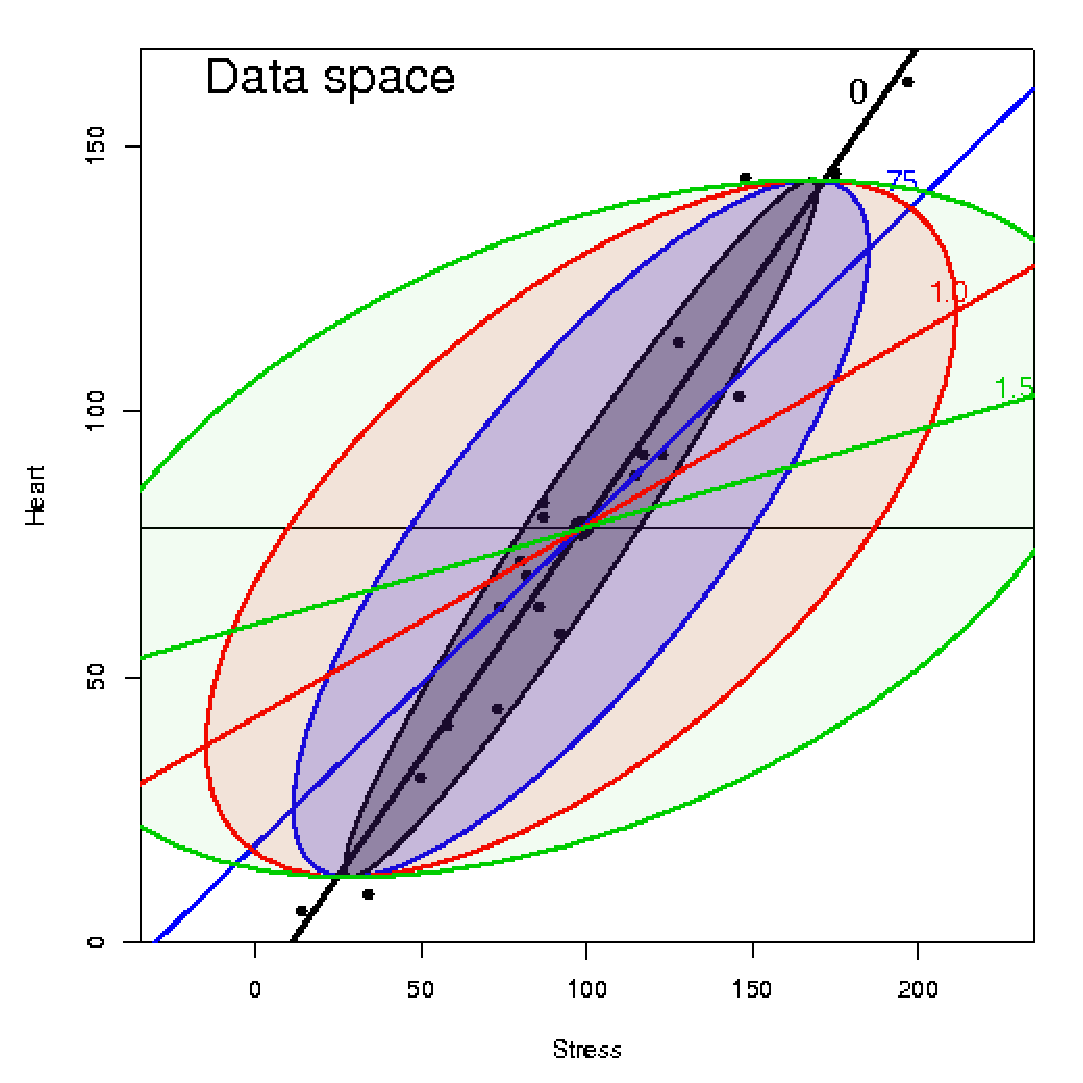
\includegraphics[width=1\linewidth]{fig/coffee-stress1}
%  \caption{}%
%  \label{fig:}
 \end{minipage}%
 \hfill
 \begin{minipage}[b]{.49\linewidth}
  \centering
  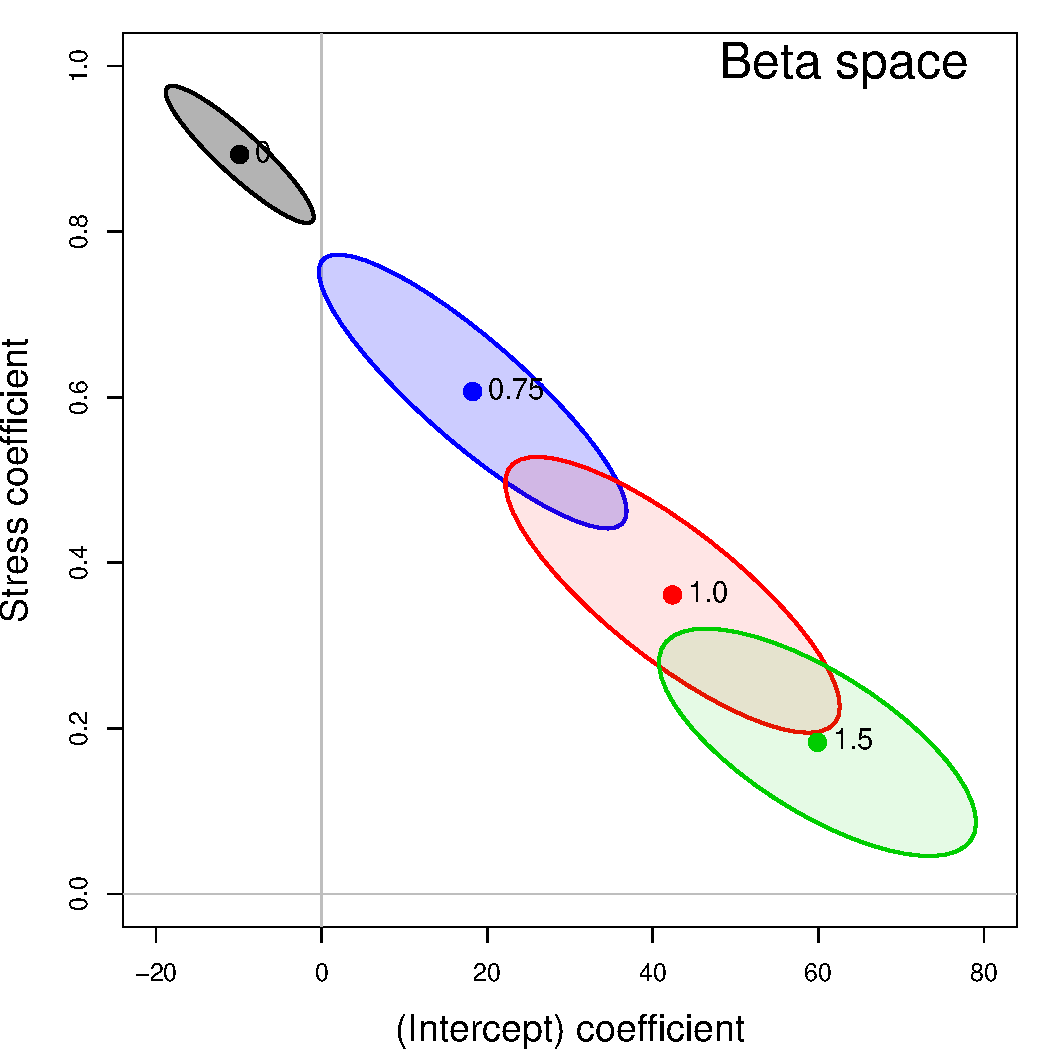
\includegraphics[width=1\linewidth]{fig/coffee-stress2}
 \end{minipage}
  \caption{Effects of measurement error in Stress on the marginal relationship between Heart disease and Stress.
  Each panel starts with the observed data ($\delta=0$), then adds random normal error,
  $\mathcal{N}(0, \delta \times \mathrm{SD}_{Stress})$, with $\delta = \{0.75, 1.0, 1.5\}$, to the value of Stress.
  Increasing measurement error biases the slope for Stress toward 0.
  Left: 50\% data ellipses; right: 50\% confidence ellipses for $(\beta_0, \beta_{Stress})$. }
  \label{fig:coffee-stress}
\end{figure}

The statistical facts are well known, though perhaps counter-intuitive in certain details:
measurement error in a predictor biases regression coefficients, while
error in the measurement in  $y$
increases the standard errors of the regression coefficients but does not introduce
bias.

% DONE
%\TODO{The rest of this section is scheduled for a rewrite (noted by John)}

In the top row of
\figref{fig:vis-reg-coffee11}, adding measurement error to the Heart disease variable
would expand the data ellipses vertically, but 
(apart from random variation)
leaves the slopes of the regression lines unchanged.
Measurement error in a predictor variable, however, biases the corresponding
estimated coefficient toward
zero (sometimes called \emph{regression attenuation}) as well as increasing standard errors.
                                         
\figref{fig:coffee-stress} demonstrates this effect for the marginal
relation between Heart disease and Stress,
with data ellipses in data space and the corresponding confidence ellipses in $\beta$ space.
Each panel starts with the observed data (the darkest ellipse, marked $0$), then adds random normal error,
$\mathcal{N}(0, \delta \times \mathrm{SD}_{Stress})$, with $\delta = \{0.75, 1.0, 1.5\}$, to the value of Stress,
while keeping the mean of Stress the same.
All of the data ellipses have the same vertical shadows ($\mathrm{SD}_{\textrm{Heart}}$), while the horizontal shadows
increase with $\delta$, driving the slope for Stress toward 0.
In $\beta$ space, it can be seen that the estimated coefficients, $(\beta_0, \beta_{\textrm{Stress}})$
vary along a line and approach $\beta_{\textrm{Stress}}=0$ for $\delta$ sufficiently large.
The vertical shadows of
ellipses for $(\beta_0, \beta_{\textrm{Stress}})$ along the $\beta_{\textrm{Stress}}$ axis
also demonstrate the effects of measurement error
on the standard error of $\beta_{\textrm{Stress}}$.

Perhaps less well-known, but both more surprising and interesting, is the effect that measurement error in one variable,
$x_1$, 
has on the estimate of the coefficient for an \emph{other} variable, $x_2$, in a multiple regression model.
\figref{fig:coffee-measerr}
shows the confidence ellipses for $(\beta_{\textrm{Coffee}}, \beta_{\textrm{Stress}})$ in the multiple regression 
predicting Heart disease, adding random normal error
$\mathcal{N}(0, \delta \times \mathrm{SD}_{Stress})$, with $\delta = \{0, 0.2, 0.4, 0.8\}$, to the value of Stress
alone.  
As can be plainly seen, while this measurement error in Stress attenuates its coefficient,
it also has the effect of biasing the coefficient for Coffee toward that in the \emph{marginal}
regression of Heart disease on Coffee alone.


\begin{figure}[htb]
  \centering
  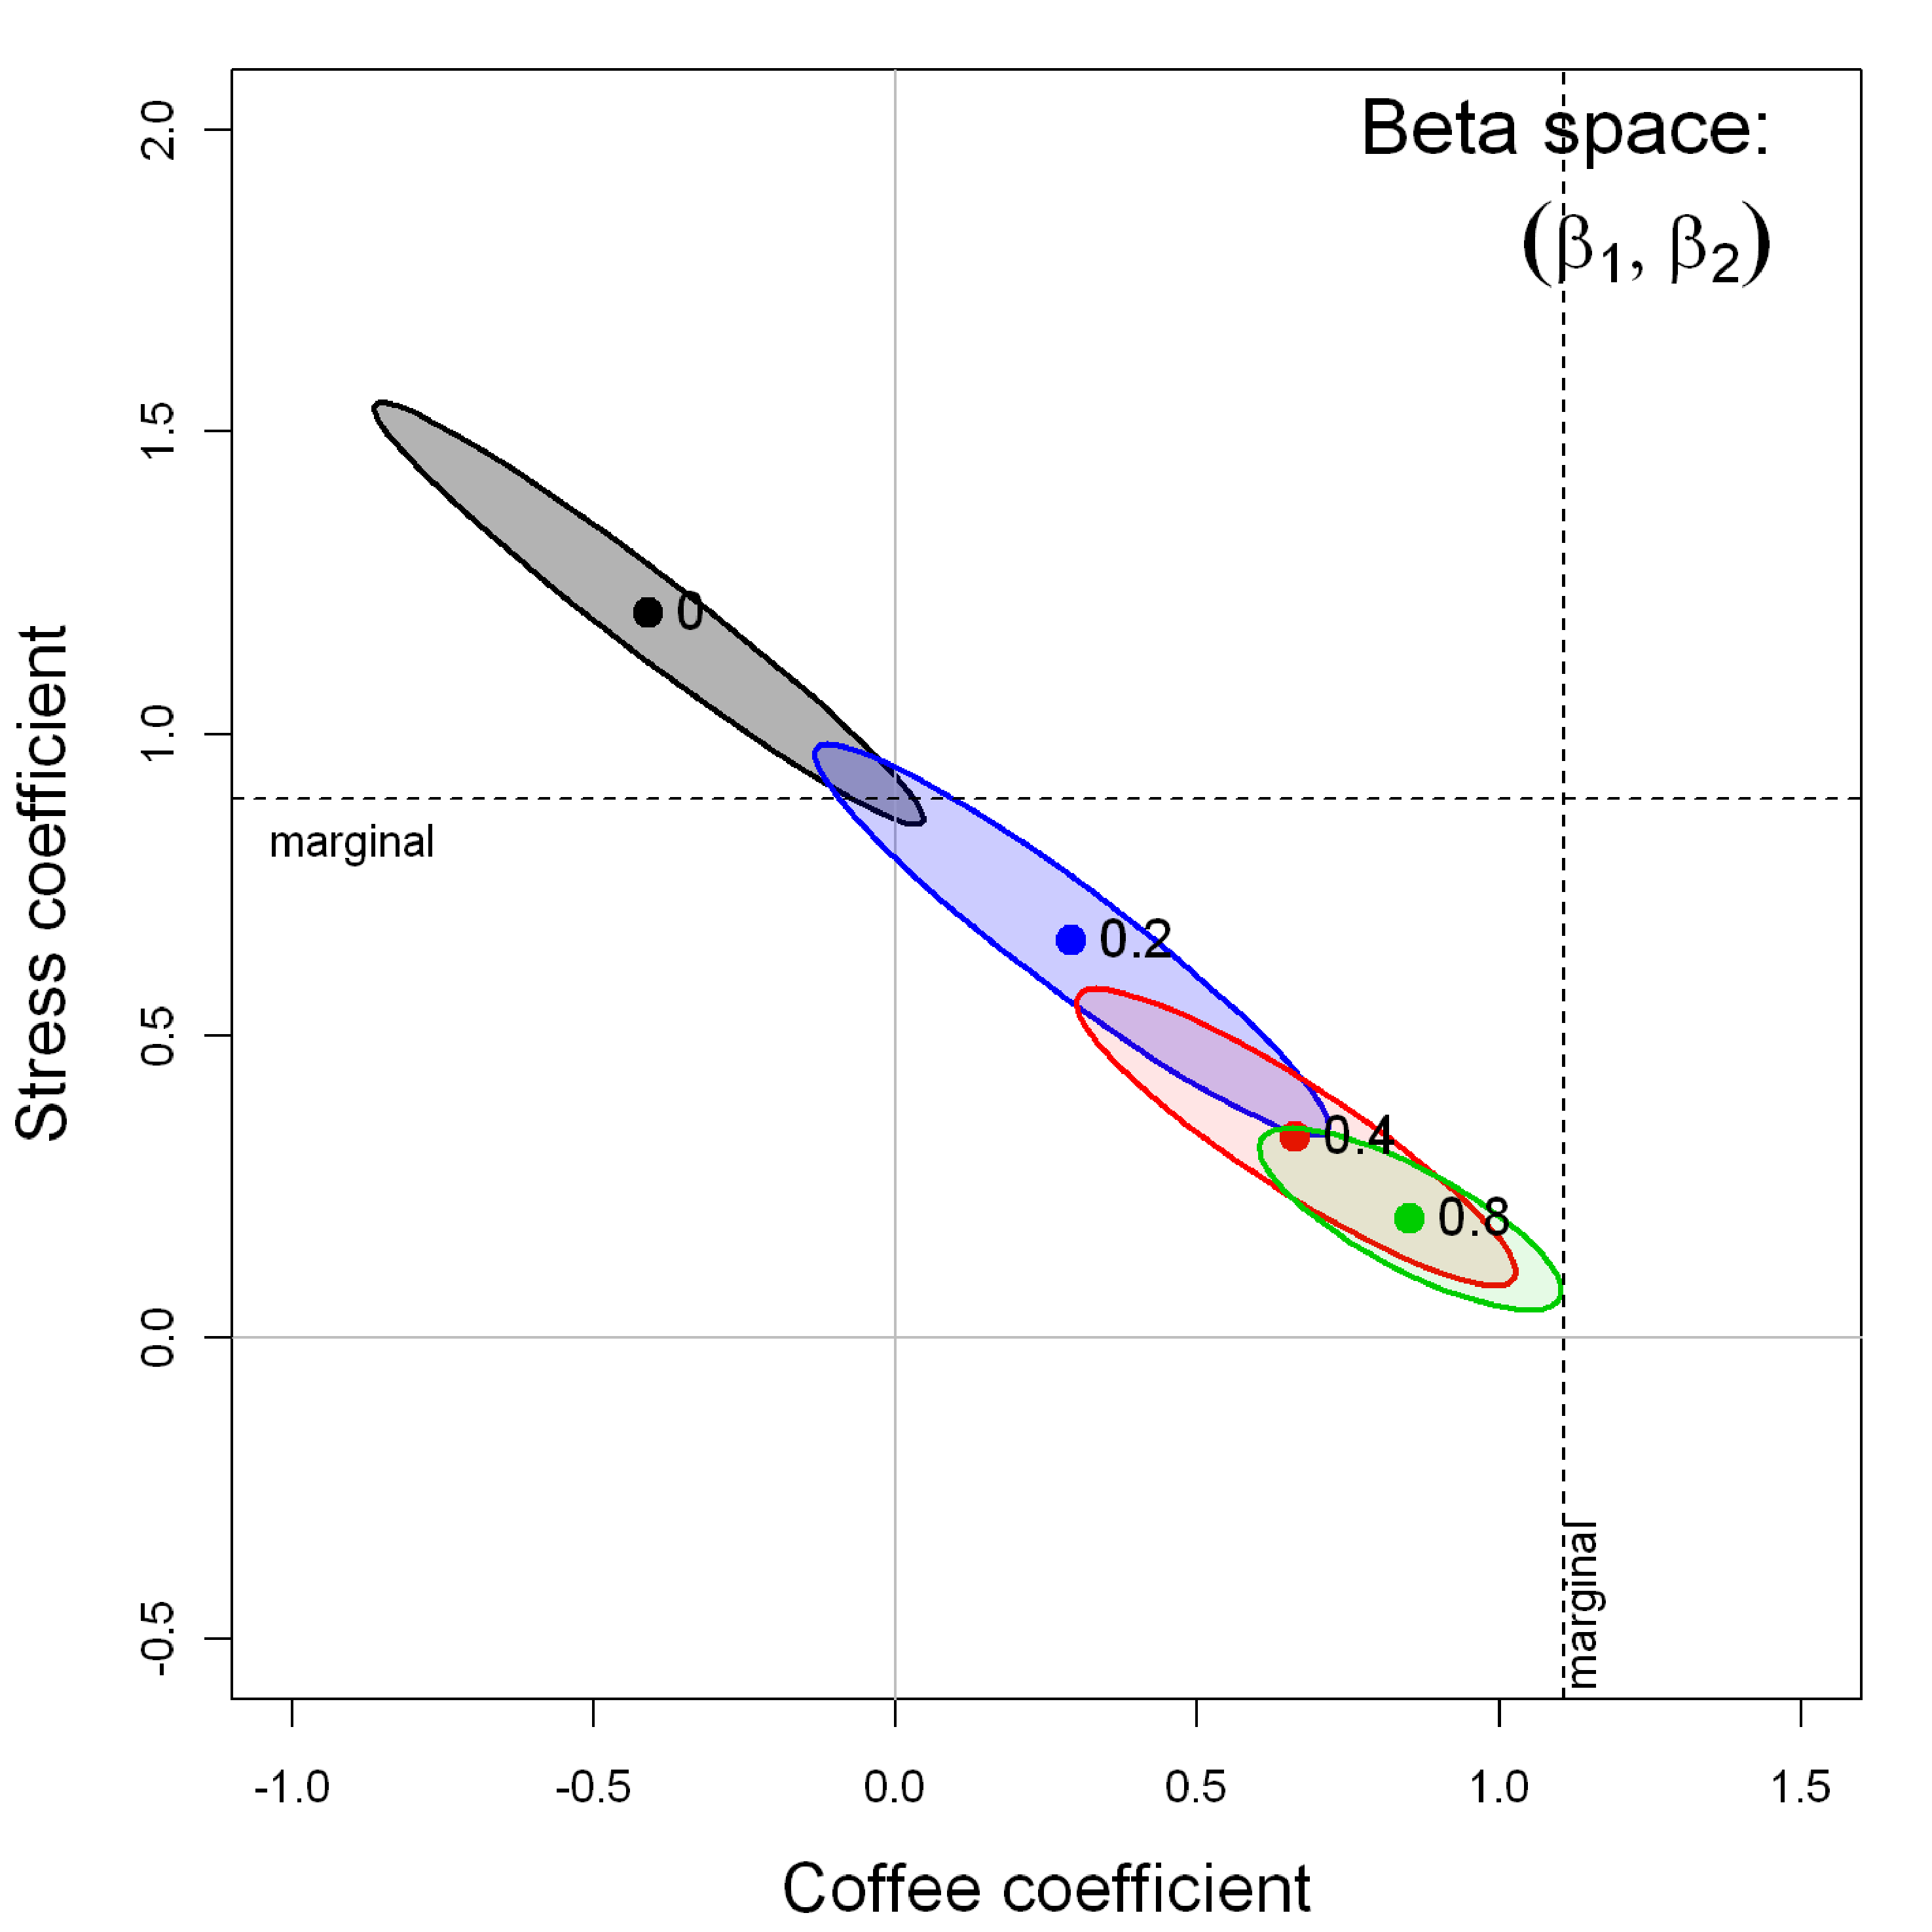
\includegraphics[width=.5\textwidth,clip]{fig/coffee-measerr}
  \caption{Biasing effect of measurement error in one variable (Stress) on on the coefficient of another variable
  (Coffee) in a multiple regression.  The coefficient for Coffee is driven towards its value in the marginal
  model using Coffee alone, as measurement error in Stress makes it less informative in the joint model.
  }%
  \label{fig:coffee-measerr}
\end{figure}

%\TODO{Can we say anything general about the relative decrease in the standard errors of $\beta_{\textrm{Coffee}}$
%with increasing error in Stress?}

%This effect is entirely understandible from a geometric perspective: increasing measurement error in $x_1$
%makes it less informative for the partial coefficient of $x_2$ 

